\documentclass[journal]{IEEEtran}
\usepackage{cite}
\usepackage{amsmath,amssymb}
\usepackage{graphicx}
\usepackage{booktabs}
\usepackage{array}
\usepackage{tikz}
\usetikzlibrary{positioning,arrows.meta,calc,fit}
\usepackage[hidelinks]{hyperref}

\newcommand{\Q}[1]{\textit{Q#1}}

\begin{document}

\title{An Entity-Transformer PPO Teacher for the Dodge Arcade Game: Evaluation Pitfalls, a Control-Frequency Surprise, and Open Questions}

\author{Taylor Turner%
\thanks{This is a working draft written to solicit feedback. Results are exploratory, come from a single training lineage, and have not been peer reviewed.}}

\markboth{Working draft: feedback requested}{Turner: An Entity-Transformer PPO Teacher for Dodge}

\maketitle

\begin{abstract}
We report an ongoing effort to train a reinforcement-learning agent for \emph{Dodge}, a small score-driven arcade game in which hazards intensify as the player scores. A deterministic Rust port feeds a vectorized environment. Our policy is a 321k-parameter entity transformer, trained with PPO from structured observations that exclude hidden state, intended as a teacher for a later vision student. After several hundred PPO updates, development means on 64 seeds rose from about 200 to 3{,}098 alive frames, but re-evaluating the retained checkpoints on 1{,}024 seeds shrank every score and reversed the ranking of the last two, a selection effect we quantify. Evaluating one frozen checkpoint with a decision on every frame instead of every fourth frame, with no retraining, raised the worst-quarter mean from 694 to 1{,}628 frames and the overall mean from 2{,}626 to 4{,}387 on fresh seeds. Opening-focused curricula and hard-seed prioritization did not help. Death telemetry on 8{,}192 fresh games shows that the anti-camping guard is almost never involved, that 91--96\% of deaths occur while a pattern is active, and that a handful of specific layouts and enemies that close in during patterns dominate. We describe the game, model, and protocol, report these results with their limits, and pose specific questions for reinforcement-learning practitioners.
\end{abstract}

\begin{IEEEkeywords}
reinforcement learning, proximal policy optimization, transformers, action repeat, evaluation methodology, arcade games
\end{IEEEkeywords}

\section{Introduction}
\IEEEPARstart{D}{odge} is a short arcade game in which the player steers a small circle around an arena, avoids moving enemies and large rectangular hazards, and scores when enemies are destroyed or pickups are collected. Scoring makes the game faster and more dangerous, so the objective that looks natural, a high score, conflicts with the one that keeps the player alive. We are building a learned agent for this game as a testbed for training a policy from structured entity observations and, later, distilling it into a student that plays from pixels.

This draft is written to share what we did and to ask for criticism. We do not present a finished or competitive agent. The best learned policy we have averages about 4{,}400 alive frames (73 seconds) in the setting we evaluate most, while a hand-written safe-powerup heuristic averages 6{,}115 on the same kind of start. The contributions we think are of interest are mostly about method rather than score:
\begin{enumerate}
\item A deterministic native port of the game with a vectorized Python environment and explicit separation of death from time-limit truncation (Sections~\ref{sec:game}--\ref{sec:model}).
\item An entity-transformer teacher and a PPO recipe with a monotone best-checkpoint retention rule (Section~\ref{sec:model}).
\item A concrete measurement lesson: a ranking made on 64 development seeds overstated every retained checkpoint's mean (re-scoring on 1{,}024 seeds lowered each by 4--16\%) and chose the wrong one of the last two, which a 2{,}048-seed confirmation corrected (Section~\ref{sec:measure}).
\item A control-frequency result: evaluating a policy trained with a four-frame action repeat using a one-frame repeat, with frozen weights, more than doubled worst-quarter survival, replicated on fresh seeds with a prespecified test (Section~\ref{sec:repeat}).
\item Null results for an opening curriculum and hard-seed prioritization, and an instrumented breakdown of where and how games end: the anti-camping guard is nearly absent from deaths, while specific patterns and enemies chasing the player during patterns account for most of them (Sections~\ref{sec:curric}--\ref{sec:telemetry}).
\end{enumerate}
Section~\ref{sec:questions} lists the questions on which we most want input.

\section{The Game}\label{sec:game}
Dodge is a port of a PICO-8 cartridge by Artridge~\cite{artridge}. The playfield is a $128\times128$ pixel square updated at 60\,Hz. The player is a circle of radius 4 px (2 px while shrunk); collisions are tested against an axis-aligned box of the same half-width. The player moves in eight directions or stays still. Movement has inertia: velocity decays, input accelerates it, and speed is capped, so the effect of an action depends on current motion.

\textit{Hazards.} Enemies enter the arena, move, grow, and collide with one another. Some chase the player. \emph{Kamikaze} enemies slow near the player and leave a growing explosion. Pattern events add large \emph{static} rectangles that charge before becoming lethal and \emph{moving} rectangles that sweep across the field. Several pattern geometries extend past the visible screen, so collision logic follows the game code rather than a clipped-screen approximation.

\textit{Scoring and pickups.} The player has no weapon. Enemies die when they collide with one another or are crushed by a pattern rectangle, and each such death adds 0.5 to the score. Three pickups also add score on contact: \emph{slow} (+1; slows the game), \emph{shrink} (+1; halves the player's radius for a while), and \emph{explode} (+1 for every enemy it destroys, which clears the screen). A pickup that clears several enemies can therefore pay more than the same enemies dying on their own. We have not measured how much of a typical game's score comes from each source.

\textit{Score-driven difficulty.} Game speed, enemy spawn timing, and pattern parameters increase with score. A policy that scores early therefore makes its own future harder. Score, shaped training reward, and survival time are related but distinct quantities, and we report them separately. Enemy deaths are the game's main source of score, but a high score is only indirectly a sign of playing well: a player who lives longer tends to score more. We therefore optimize and report survival (alive frames) rather than score.

\textit{Anti-camping guard.} If the player remains inside a central region for more than 50 consecutive frames, the game spawns extra enemies at the corners (the cartridge routine \texttt{fyou}); leaving the region resets the counter. This is a native mechanic. We add no center-avoidance penalty.

\textit{Death.} A game ends on the first lethal contact. We record the first contact's class: normal enemy, kamikaze body, kamikaze explosion, static rectangle, or moving rectangle. A full game runs until death or an 18{,}000-frame cap (300 seconds), excluding 13 menu frames.

\section{Environment and Observations}\label{sec:env}
\textit{Simulator.} The deterministic game core is written in Rust and stepped headlessly. Headless stepping preserves the draw-time random-number consumption of the original so trajectories remain aligned with the cartridge. A vectorized wrapper exposes batched environments to Python through PyO3.

\textit{Units.} A \emph{frame} is one 1/60\,s update. A \emph{decision} is one policy action, held for $K$ frames; the default is $K=4$ (15 decisions per second). If death occurs inside a repeat, stepping stops at that frame. The discount $\gamma=0.995$ and the GAE decay are defined per decision, not per frame.

\textit{Observation.} The structured observation is a global record of 14 features (player position, velocity, size, score, game speed, boundary distances) and up to 80 entity slots with 16 features each (relative geometry, signed collision gaps, motion, hazard-timing estimates), together with an entity-type ID in $\{1,\dots,8\}$ for each slot and a validity mask (Table~\ref{tab:obs}). The mask has one entry per slot: 1 if the slot holds an entity currently on screen, 0 if it is empty padding. Most games have far fewer than 80 entities, so most slots are empty. The agent never sees seed identifiers, hidden timers, the random-number state, or future pattern schedules. This \emph{non-clairvoyance} rule keeps the teacher's inputs within what a vision student could in principle infer from short frame history.

\begin{table}[t]
\caption{Policy inputs and outputs.}\label{tab:obs}
\centering
\small
\begin{tabular}{@{}ll@{}}
\toprule
Item & Content \\
\midrule
Global token & 14 floats \\
Entity slots & 80 $\times$ 16 floats, type ID $\in\{1..8\}$, validity mask (1 = entity, 0 = empty) \\
Actions & 9 (neutral, 4 cardinal, 4 diagonal) \\
Value output & 1 scalar \\
Frame cap & 18{,}000 gameplay frames \\
\bottomrule
\end{tabular}
\end{table}

\textit{Reward.} One decision executes $K$ frames. Its reward is the score gained during those frames, plus 0.01 for each frame the player stays alive, minus 5 if the player dies during them. The PPO code then multiplies the reward by 0.1. An episode can end in two different ways, and we treat them differently~\cite{pardo2018time}. \emph{Death} is a true ending: no further reward can follow, so the value of the state after death is set to zero. A \emph{truncation} happens when we stop a game that is still going, at the 18{,}000-frame cap or at a shorter cutoff used in some runs. The player could have kept collecting reward, so we do not set the final value to zero; the critic's own estimate of that last state is used instead (this is called bootstrapping).

\section{Model and Training}\label{sec:model}
\textit{Architecture.} The teacher is an entity transformer~\cite{vaswani2017attention} with 81 tokens: one global token and 80 entity slots (Fig.~\ref{fig:arch}). The global features pass through a linear projection; each entity passes through a two-layer MLP and adds a learned type embedding. Two pre-norm self-attention blocks (width 128, four heads, feed-forward width 256, GELU) process all tokens, with empty slots masked out so that attention ignores them. The actor and critic are separate two-layer MLP heads on the global token's output, giving nine logits and one value. The model has 321{,}290 parameters.

\begin{figure}[t]
\centering
\resizebox{\columnwidth}{!}{%
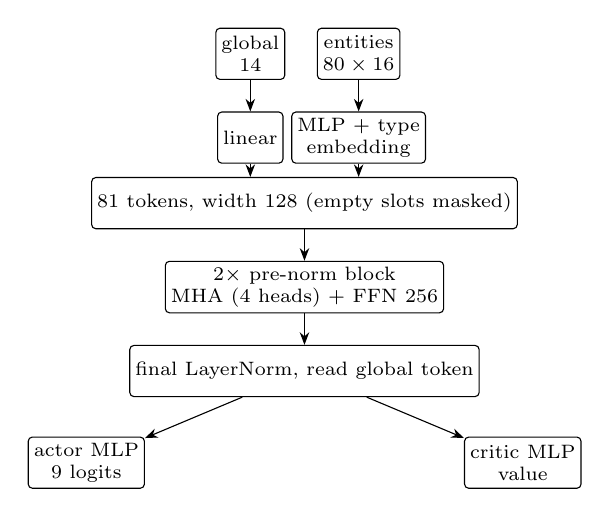
\begin{tikzpicture}[
  box/.style={draw, rounded corners=1.5pt, minimum height=6.5mm, align=center, font=\scriptsize, inner sep=2pt},
  arr/.style={-{Stealth[length=1.6mm]}, thin},
  node distance=4mm]
  \node[box] (g) {global\\14};
  \node[box, right=of g] (e) {entities\\$80\times16$};
  \node[box, below=4mm of g] (gp) {linear};
  \node[box, below=4mm of e] (ep) {MLP + type\\embedding};
  \node[box, below=5mm of $(gp)!0.5!(ep)$, minimum width=3.4cm] (tok) {81 tokens, width 128 (empty slots masked)};
  \node[box, below=4mm of tok, minimum width=3.4cm] (tf) {2$\times$ pre-norm block\\MHA (4 heads) + FFN 256};
  \node[box, below=4mm of tf, minimum width=3.4cm] (ln) {final LayerNorm, read global token};
  \node[box, below left=5mm and -2mm of ln] (a) {actor MLP\\9 logits};
  \node[box, below right=5mm and -2mm of ln] (c) {critic MLP\\value};
  \draw[arr] (g) -- (gp); \draw[arr] (e) -- (ep);
  \draw[arr] (gp.south) -- (gp.south |- tok.north);
  \draw[arr] (ep.south) -- (ep.south |- tok.north);
  \draw[arr] (tok) -- (tf); \draw[arr] (tf) -- (ln);
  \draw[arr] (ln) -- (a); \draw[arr] (ln) -- (c);
\end{tikzpicture}}
\caption{Entity-transformer teacher. Both heads read the global token after two attention blocks.}\label{fig:arch}
\end{figure}

\textit{PPO.} We use PPO~\cite{schulman2017ppo} with GAE~\cite{schulman2016gae}. Each update collects 256 decisions from each of 64 environments (16{,}384 transitions) and runs four epochs over minibatches of 512, with an early-stop KL threshold. Table~\ref{tab:ppo} lists the settings. The learning rate was lowered in stages from $3\times10^{-4}$ to $1\times10^{-4}$ to $3\times10^{-5}$; all later experiments use the last value unless stated. Episodes in flight are abandoned at fixed segment boundaries every 60 updates while model, optimizer, and random-number state continue.

\begin{table}[t]
\caption{PPO settings.}\label{tab:ppo}
\centering
\small
\begin{tabular}{@{}ll@{}}
\toprule
Setting & Value \\
\midrule
Discount $\gamma$, GAE $\lambda$ & 0.995, 0.95 \\
Clip, entropy coef., value coef. & 0.2, 0.01, 0.5 \\
Epochs, minibatch, grad-norm clip & 4, 512, 0.5 \\
Rollout & 64 envs $\times$ 256 decisions \\
Target KL (epoch early stop) & 0.03 \\
Learning rate (later experiments) & $3\times10^{-5}$ \\
Reward scale & 0.1 \\
\bottomrule
\end{tabular}
\end{table}

\textit{Curriculum.} Training first used a difficulty-1 stage without patterns (2{,}000-frame cap), then difficulty~2 with patterns and powerups on, with an 18{,}000-frame cap. Entering difficulty~2 collapsed performance: 42 of 64 evaluation games ended before the first pattern appeared, plausibly because the pattern embeddings had never been trained.

\textit{Retention rule.} After the plateau in Section~\ref{sec:measure}, a candidate becomes the retained best only if it improves the development mean after audit. Retention restores model, Adam, and RNG state. In the runs we inspected, the final checkpoint was worse than the best intermediate one, so retention produced the last four gains.

\section{Evaluation Protocol}\label{sec:protocol}
All numbers are alive frames at 60\,Hz, difficulty~2, patterns and powerups on, cap 18{,}000, unless stated. We report \emph{Worst} and \emph{Best} (single games), \emph{Mean}, and two quarter means: \Q{1} is the mean of the worst 25\% of games and \Q{4} the mean of the best 25\%. \Q{1} is not the 25th percentile. We make the lower tail the primary concern because the mean can rise while weak games get worse. \emph{Argmax} evaluation chooses the highest-probability action; \emph{sampled} evaluation draws from the policy. \emph{Development} cohorts are used to rank and tune; \emph{confirmation} cohorts are drawn fresh and used once after choices are fixed. The minimum paired difference we can resolve with 64 seeds and one training seed is about 620 frames, which is larger than several of the gains we initially accepted.

\section{Results}\label{sec:results}
\subsection{Progress and the 64-seed selection effect}\label{sec:measure}
Fig.~\ref{fig:progress}(a) shows the development mean over time. The first learned policies stayed near the 100--250 frame level of a random policy (255 frames). After the curriculum and difficulty-2 entry, means rose and then plateaued at 1{,}100--1{,}900 across many runs, a period in which much of the effort was lost to harness and guard failures. A first mean above 2{,}000 (2{,}240, best of 24 evaluations) was not sustained. A monotone best-checkpoint rule and learning-rate drops then produced a retained sequence (Table~\ref{tab:retained}) whose 64-seed means rose from 1{,}854 to 3{,}098. Per-step gains shrank: $+29.3\%$, $+8.9\%$, $+8.7\%$, $+5.4\%$.

\begin{figure*}[t]
\centering
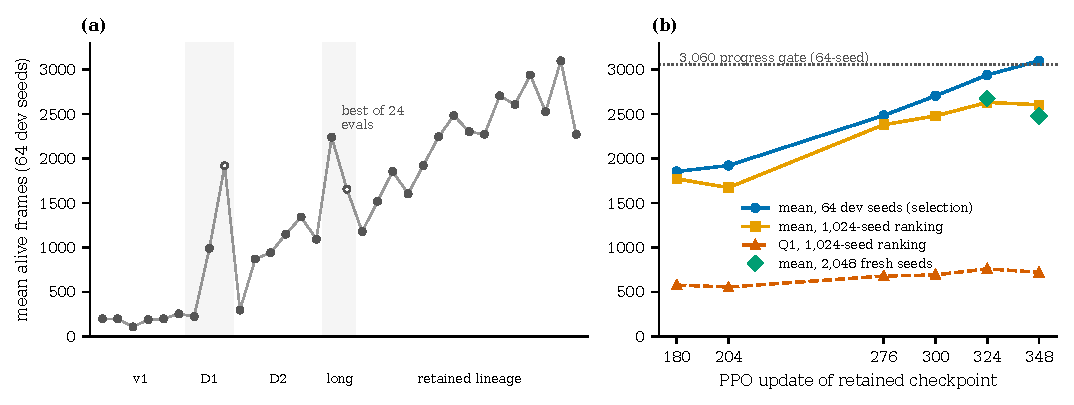
\includegraphics[width=\textwidth]{figs/progress.pdf}
\caption{(a) Development mean alive frames in evaluation order for all teacher runs (hollow: capped at 2{,}000 frames or a run's endpoint). (b) The six retained checkpoints scored on 64 development seeds (the selection cohort), re-scored on 1{,}024 ranking seeds, and checkpoints 324 and 348 scored on 2{,}048 fresh seeds. Every retained score fell on the larger cohort. The 3{,}060 gate is a 64-seed criterion.}\label{fig:progress}
\end{figure*}

We then re-scored the six retained checkpoints on 1{,}024 frozen seeds, with no logged overlap with training or selection seeds (coverage of the logs is not proven complete). Every mean fell, by 4--16\% (Fig.~\ref{fig:progress}b, Table~\ref{tab:retained}), and the order of the last two changed: checkpoint 324 (2{,}631) edged 348 (2{,}604) on ranking. On 2{,}048 further fresh seeds, 324 beat 348 by 195.7 frames (7.9\%; one-sided 95\% bootstrap lower bound $+109$ frames, resampling by seed). The confirmed values for 324 are Worst 350, \Q{1} 774, Mean 2{,}673, \Q{4} 5{,}071, Best 10{,}730. We read this as a selection effect: choosing the best of many candidates on 64 reused seeds inflates the winner's score and can pick the wrong candidate. The learning curve itself survives the correction (180$\to$324 rises 1{,}772$\to$2{,}631 on 1{,}024 seeds, about 48\%, against about 59\% on 64 seeds), but it is flatter than first reported, and the last step was noise.

\begin{table}[t]
\caption{Retained checkpoints on the selection cohort (64 seeds) and on 1{,}024 ranking seeds.}\label{tab:retained}
\centering
\small
\begin{tabular}{@{}rrrrr@{}}
\toprule
Update & Mean (64) & Mean (1{,}024) & \Q{1} (1{,}024) & \Q{4} (1{,}024) \\
\midrule
180 & 1{,}854 & 1{,}772 & 577 & 3{,}565 \\
204 & 1{,}921 & 1{,}673 & 556 & 3{,}499 \\
276 & 2{,}484 & 2{,}380 & 679 & 4{,}650 \\
300 & 2{,}704 & 2{,}478 & 691 & 4{,}778 \\
324 & 2{,}939 & 2{,}631 & 760 & 4{,}945 \\
348 & 3{,}098 & 2{,}604 & 720 & 4{,}905 \\
\bottomrule
\end{tabular}
\end{table}

Two further observations motivate the lower-tail focus. On the 64-seed cohort \Q{1} stayed between 567 and 870 frames while \Q{4} grew from about 2{,}300 to 6{,}000. Even the best checkpoint's worst quarter averages under 800 frames.

\subsection{Continued training}\label{sec:continue}
Starting from a candidate built on checkpoint 324 (60 further updates, selected by \Q{1} after exploratory comparison, not by a preregistered rule), we ran 600 more updates at a constant rate $3\times10^{-5}$, evaluating every 60 updates on a new 1{,}024-seed cohort (Fig.~\ref{fig:contdec}a). The mean rose from 2{,}162 to 2{,}702 at update 600 ($+25\%$) and \Q{1} from 646 to 732 at update 420 ($+13\%$), with considerable checkpoint-to-checkpoint noise: update 420 had the best \Q{1} and update 600 the best mean. More training helped, slowly, and the lower tail barely moved. (This cohort differs from the ranking cohort, so levels are not directly comparable across Table~\ref{tab:retained} and Fig.~\ref{fig:contdec}a.)

\begin{figure*}[t]
\centering
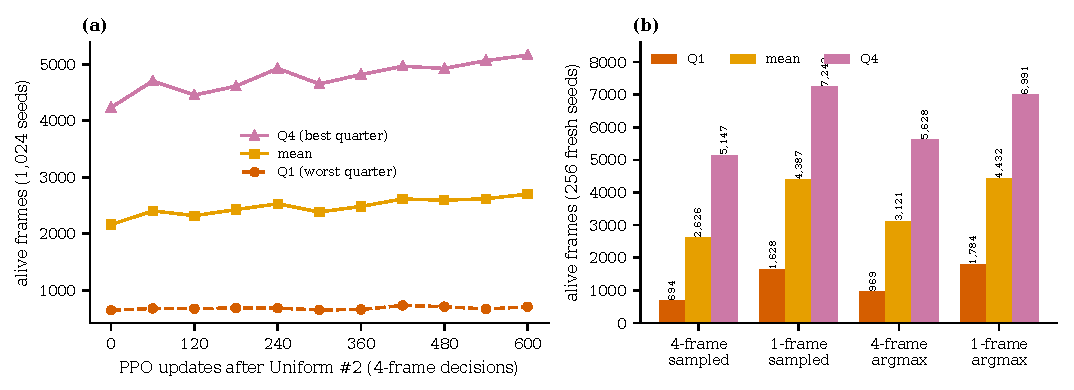
\includegraphics[width=\textwidth]{figs/continuation_decisions.pdf}
\caption{(a) 600-update continuation with four-frame decisions on a 1{,}024-seed cohort. (b) One frozen checkpoint (update 420), four versus one frame per decision, on 256 fresh seeds (sampled settings pool three repetitions, 768 games). \Q{1} is the mean of the worst 25\% of games.}\label{fig:contdec}
\end{figure*}

\subsection{Decision frequency}\label{sec:repeat}
The policy was trained with $K=4$. We evaluated the frozen update-420 checkpoint with $K=1$ (a decision every frame), changing nothing else, in a $2\times2$ design with action mode (sampled or argmax). A first screen (256 seeds, sampled conditions repeated three times) and a prespecified confirmation on 256 new seeds agreed (Table~\ref{tab:repeat}, Fig.~\ref{fig:contdec}b). With sampled actions, \Q{1} rose from 694 to 1{,}628 frames and the mean from 2{,}626 to 4{,}387. The prespecified contrast, sampled $K{=}1$ minus $K{=}4$ on \Q{1}, was $+934$ frames with a 95\% interval of $+767$ to $+1{,}114$ (bootstrap by seed cluster, keeping the three repetitions of each seed together). The screen gave $+914$ ($+728$ to $+1{,}094$). Under argmax the same direction held ($+813$, $+423$ to $+1{,}210$). The advantage of argmax over sampling was $+275$ ($+63$ to $+497$) at $K{=}4$ and $+160$ ($-197$ to $+531$) at $K{=}1$; the interaction contrast ($-117$, $-534$ to $+313$) is not resolved.

Survival curves (Fig.~\ref{fig:milestones}) show the effect on every horizon: at $K{=}1$, 94\% of games pass 1{,}000 frames versus 77\% at $K{=}4$, and the median game survives about 4{,}400 frames versus about 2{,}300. With $K{=}1$ the best single game on fresh seeds reached 11{,}999 (sampled) and 12{,}480 (argmax) frames.

\begin{table}[t]
\caption{Checkpoint 420, frozen weights, 256 fresh confirmation seeds. Mean / \Q{1} / \Q{4} in alive frames.}\label{tab:repeat}
\centering
\small
\begin{tabular}{@{}llrrrr@{}}
\toprule
Mode & $K$ & Mean & \Q{1} & \Q{4} & Best \\
\midrule
sampled & 4 & 2{,}626 & 694 & 5{,}147 & 8{,}866 \\
sampled & 1 & 4{,}387 & 1{,}628 & 7{,}243 & 11{,}999 \\
argmax & 4 & 3{,}121 & 969 & 5{,}629 & 9{,}682 \\
argmax & 1 & 4{,}432 & 1{,}784 & 6{,}991 & 12{,}480 \\
\bottomrule
\end{tabular}
\end{table}

\begin{figure}[t]
\centering
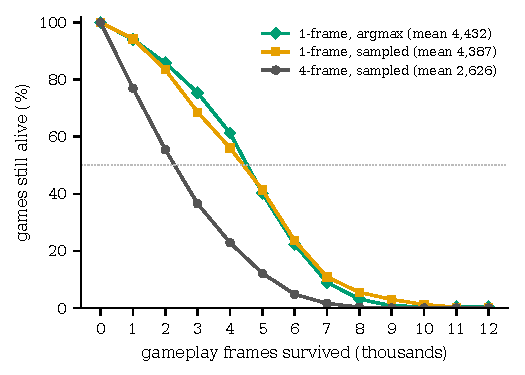
\includegraphics[width=\columnwidth]{figs/milestones.pdf}
\caption{Share of games still alive at each 1{,}000-frame milestone (checkpoint 420, fresh seeds; sampled lines pool 768 games, argmax 256).}\label{fig:milestones}
\end{figure}

Caveats are important here. This is one checkpoint from one training lineage and 256 seeds; the three repetitions of the sampled conditions are not independent training replicas. The policy was never trained at $K=1$, so we do not know whether the gain reflects finer control, shorter reaction delay (up to 66.7\,ms at $K{=}4$ versus 16.7\,ms), changed discount and GAE time scales, or an interaction of velocity features and inertia with the changed observation cadence. A $K{=}1$ evaluation costs five to six times as much wall-clock time. Training with $K{=}1$ under matched frame budgets, with $\gamma$ and $\lambda$ rescaled to preserve their horizon in game time, is the obvious next experiment.

\subsection{Opening curriculum and hard-seed prioritization}\label{sec:curric}
Because weak games dominate the lower tail, we tried two interventions aimed at opening survival, each as matched training pairs from a common parent. A mixture that ran 70\% of training episodes at a 1{,}000-frame opening stage and 30\% as full games gave opening survival (reaching 1{,}000 frames) of 70.4\% for the control and 72.3\% for the curriculum, with pair differences of $+6.5$, $+0.8$, and $-1.6$ points and mixed changes in the mean ($+146$, $-141$, $-33$ frames). No replica advanced past its first 1{,}000-frame stage. A second test sampled training seeds from a frozen pool of 512 seeds, half where an earlier policy died before 1{,}000 frames and half where it survived longer, with prioritization drawing about 75\% of starts from the hard half (cf.~\cite{jiang2021plr}). In all three pairs the prioritized policy had lower \Q{1}; averaged over pairs it was 35 frames lower in \Q{1} and 65 frames lower in mean (Table~\ref{tab:priority}). With three pairs we read these as ``no benefit observed'' rather than as evidence of harm. A later diagnostic suggested that an earlier curriculum recipe gave about half as many post-1{,}000-frame decisions, which motivated a plan we have not yet run: full games with seed priority that preserves late-game exposure.

\begin{table}[t]
\caption{Six policies, 60 updates each, sampled actions, 1{,}024 seeds. Pairs share parent and training randomness.}\label{tab:priority}
\centering
\small
\begin{tabular}{@{}rlrrrr@{}}
\toprule
Pair & Sampling & Worst & \Q{1} & Mean & \Q{4} \\
\midrule
1 & uniform & 89 & 658 & 2{,}236 & 4{,}392 \\
1 & hard-priority & 125 & 606 & 2{,}077 & 4{,}127 \\
2 & uniform & 225 & 664 & 2{,}208 & 4{,}264 \\
2 & hard-priority & 153 & 618 & 2{,}205 & 4{,}244 \\
3 & uniform & 153 & 626 & 2{,}142 & 4{,}215 \\
3 & hard-priority & 136 & 617 & 2{,}108 & 4{,}139 \\
\bottomrule
\end{tabular}
\end{table}

\subsection{Where games end}\label{sec:deaths}
Fig.~\ref{fig:deaths} splits the first lethal contact by the window in which the game ended, for sampled actions at $K{=}4$ and $K{=}1$ (768 fresh games each). Normal enemies account for 46--68\% of deaths in every window. At $K{=}1$ far fewer games end early (5.7\% before 1{,}000 frames versus 23\%), and the early deaths that remain are disproportionately moving rectangles (27\% versus 16\%). Static rectangles account for about 30\% of deaths past 3{,}000 frames, consistent with a harder pattern phase. These breakdowns are descriptive. The saved game records distinguish only the five contact classes, so they cannot say how many normal-enemy deaths involve enemies spawned by the anti-camping guard, or which individual patterns, rather than ``a rectangle'', are lethal and when. Section~\ref{sec:telemetry} adds that telemetry.

\begin{figure*}[t]
\centering
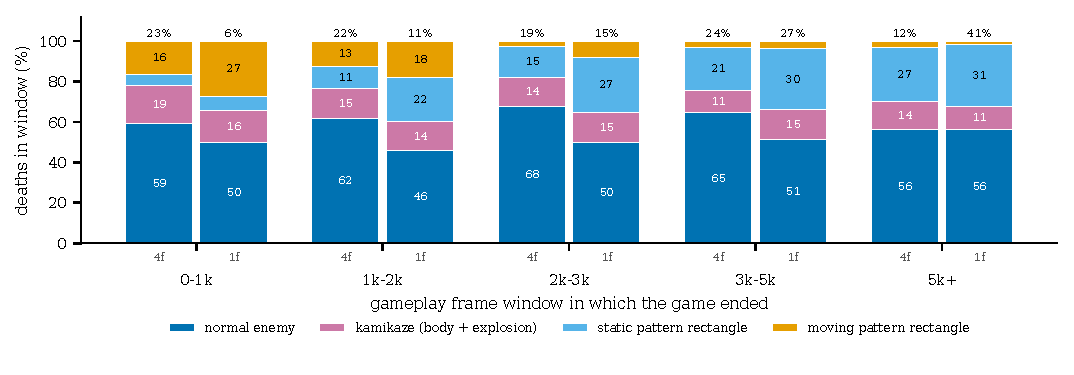
\includegraphics[width=\textwidth]{figs/death_causes.pdf}
\caption{First lethal contact by the window in which the game ended, checkpoint 420, sampled actions, 768 fresh games per setting (4f: $K{=}4$; 1f: $K{=}1$). The percentage above each bar is that window's share of all games.}\label{fig:deaths}
\end{figure*}

\subsection{Death telemetry: guard, patterns, and enemies}\label{sec:telemetry}
We added an observation-only recorder to the game core: it is off by default, absent from snapshots, and never touches the random number generator, reward, or any policy input. It logs every anti-camping (``fyou'') trigger and the enemies it spawns, every pattern encounter (identifier, type, start, end), and at the first lethal contact the killer's provenance and age, the active pattern and its age, the player's position, and the other enemies on screen. Before reading any trace we replayed the saved checkpoint-420 evaluations with the new build: all 2{,}048 saved games (eight groups: argmax and sampled, $K{=}1$ and $K{=}4$) matched in alive frames, cause and fatal frame, with zero mismatches. We then ran 2{,}048 fresh seeds in each of four settings (argmax and sampled, $K{=}1$ and $K{=}4$). All 8{,}192 games ended in death; none reached the cap. Below we use the argmax runs; intervals are 95\% bootstrap intervals over seeds. A prespecified prediction that at least 40\% of $K{=}4$ deaths before 1{,}000 frames would follow a guard trigger was false.

\textit{The guard is not the cause.} Only 2.9\% of $K{=}1$ and 1.1\% of $K{=}4$ games ever triggered it, and 0.4--3.8\% of deaths in each window followed a trigger. Enemies spawned by the guard were the killer in 7 of 1{,}227 enemy kills at $K{=}1$ and 4 of 1{,}398 at $K{=}4$, so the 40--60\% normal-enemy share (Fig.~\ref{fig:deaths}) is ordinary spawns. Deaths in the 300 frames after a trigger were 27 against 6.9 expected (3.9$\times$, [2.6, 5.7], pooled), but this rests on 27 deaths, touches under 3\% of games, and is observational.

\textit{Patterns are where games end.} A pattern is active in 42--49\% of frames but in 91--96\% of $K{=}1$ deaths (88--94\% at $K{=}4$) (Fig.~\ref{fig:telehazard}b); the per-frame death rate with a pattern active is 14--27$\times$ higher at $K{=}1$ and 10--20$\times$ higher at $K{=}4$. Decision frequency lowers the hazard in every window before 5{,}000 frames (Fig.~\ref{fig:telehazard}a; for example 6.3\% [5.2, 7.4] versus 13.9\% [12.5, 15.5] of games die before frame 1{,}000), but the pattern effect is present at both. Lethality is concentrated in specific layouts (Fig.~\ref{fig:telepatterns}). Pattern 28 is the largest early killer (22\% of $K{=}1$ and 20\% of $K{=}4$ deaths before 1{,}000 frames, but only 15\% and 28\% of its encounters end in death), while pattern 3 kills in 70\% ($K{=}1$) and 74\% ($K{=}4$) of encounters and pattern~4, its transposed layout, in 40\% and 57\%. Score-gated patterns 13, 14, 25 and 26 were survived in 1 of 355 encounters at $K{=}1$ and 0 of 155 at $K{=}4$, yet only 15--47\% of those deaths were rectangle contact. The five most lethal identifiers hold only 41--44\% of rectangle kills, so no short list of patterns accounts for the failures.

\textit{The policy loses to enemies while patterns are active.} At $K{=}1$, enemy-contact deaths occur about 11 times as often per frame while a pattern is active (0.27 versus 0.02 per 1{,}000 frames), and more often than rectangle contact (0.20). In a second $K{=}4$ pass with per-frame paths on the same seeds (reproducing the first pass exactly), the 1{,}371 enemy-contact deaths show a steady approach (Fig.~\ref{fig:teleapproach}): enemies home on the player at roughly 0.8--0.95 px per frame, the player's median retreat is slower than that, and in the last 10--15 frames its median motion turns toward the killer. Paths into the worst static patterns (Fig.~\ref{fig:telepaths}) suggest two recurring shapes: running along a wall into a rectangle that touches it (patterns 3 and 39), and circling inside the four-rectangle cross of pattern 28 until an enemy arrives. Pattern 4 has the same rectangles as 3 in a transposed layout but its deaths are spread out.

These are associations at the death frame. They have no counterfactual: we cannot say the policy ``should'' have turned away, and rectangle coverage does not predict lethality (correlation 0.11). Death position and enemy count have no base rate in the data. The path pass exists only at $K{=}4$, because the $K{=}1$ pass was stopped by the power guard. Everything is one checkpoint on one seed block, and the guard counts are small. Distinguishing a perception failure from a planning failure needs counterfactual branching: restore a state about 60 frames before death and vary the actions.

\begin{figure*}[t]
\centering
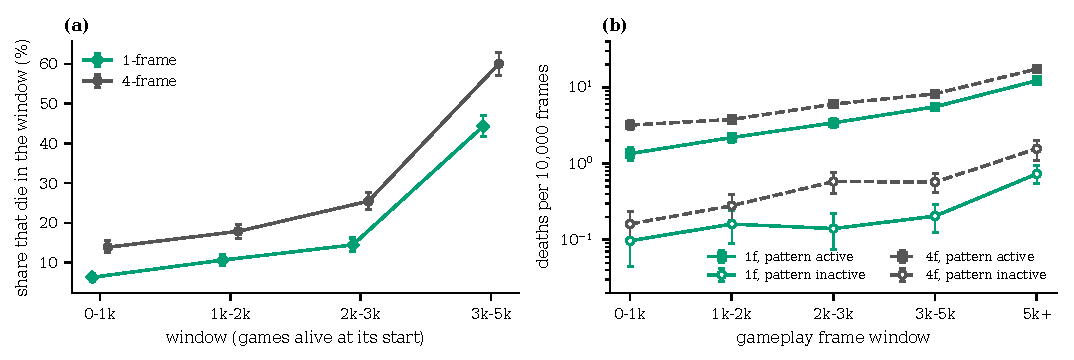
\includegraphics[width=\textwidth]{figs/tele_hazard.pdf}
\caption{Checkpoint 420, argmax, 2{,}048 fresh seeds. (a) Share of games alive at the start of each window that die in it, $K{=}1$ versus $K{=}4$ (the 5k+ window is 100\% by construction because no game reached the cap). (b) Deaths per 10{,}000 frames lived with a pattern active versus inactive, log scale. Bars are 95\% bootstrap intervals over seeds.}\label{fig:telehazard}
\end{figure*}

\begin{figure*}[t]
\centering
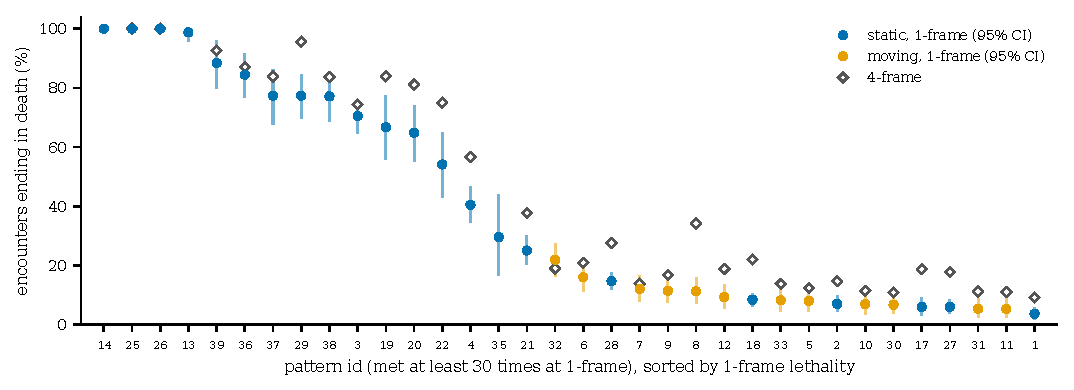
\includegraphics[width=\textwidth]{figs/tele_patterns.pdf}
\caption{Share of encounters with each pattern during which the player died, for patterns met at least 30 times at $K{=}1$ (filled, with 95\% intervals) and the same at $K{=}4$ (hollow). Ids 13, 14, 25, 26 and the 36--39 family are almost always fatal; pattern 3 is fatal far more often than its transposed layout, pattern 4. Score-gated patterns appear only late in a game, so cross-identifier comparisons mix lethality with exposure at higher score.}\label{fig:telepatterns}
\end{figure*}

\begin{figure*}[t]
\centering
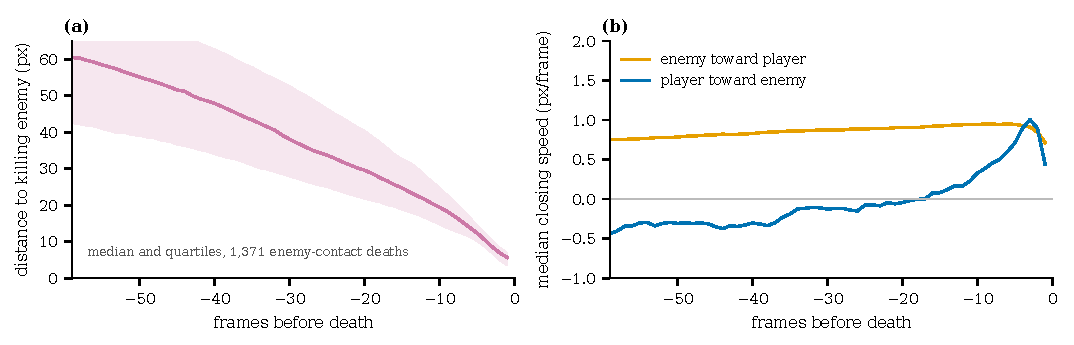
\includegraphics[width=\textwidth]{figs/tele_approach.pdf}
\caption{The 1{,}371 enemy-contact deaths in the $K{=}4$ argmax path pass. (a) Median distance to the killing enemy, with quartiles. (b) Median speed along the line to the killer; negative player speed is retreat.}\label{fig:teleapproach}
\end{figure*}

\begin{figure*}[t]
\centering
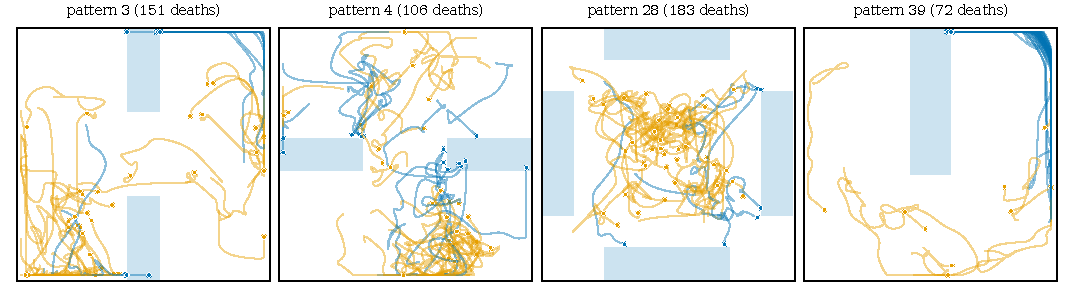
\includegraphics[width=\textwidth]{figs/tele_paths.pdf}
\caption{Last 60 frames before death inside four static patterns ($K{=}4$ argmax; first 45 qualifying deaths per pattern; blue: died to the rectangle, orange: died to an enemy; dots mark the death position; shaded: the pattern's lethal rectangles). Deaths are those with that pattern active at the fatal frame, not caused by a moving rectangle, and with every recorded rectangle lethal. Each path is the player's recorded centre over the last 60 frames. An interactive version covering every pattern id and every death that occurred while a pattern was active (1{,}881 deaths) is in \texttt{figs/death\_paths.html}.}\label{fig:telepaths}
\end{figure*}

\section{Limitations}\label{sec:limits}
\textit{One lineage.} All checkpoints descend from a single training lineage; nearly every comparison involves one or three training seeds, and evaluation seeds do not substitute for training replicas. \textit{Exploratory selection.} Several choices (continuation start, which checkpoint to freeze) were made after looking at results, not preregistered; the $K{=}1$ confirmation is the main prespecified test. \textit{Cohorts.} Cohorts differ across sections, so levels are comparable only within a section. \textit{No explanation.} We have no demonstrated mechanism for the plateau, for the $K{=}1$ gain, or for why intermediate checkpoints beat run endpoints; the death telemetry (Section~\ref{sec:telemetry}) is descriptive, covers one checkpoint, and has no counterfactuals. \textit{Baseline.} The heuristic baseline (6{,}115 mean frames over 1{,}000 episodes, 15 reaching the cap) still beats every learned policy on mean. \textit{Vision.} No student has been trained; the teacher/student claim is a plan.

\section{Questions for Practitioners}\label{sec:questions}
We would especially value opinions on the following.
\begin{enumerate}
\item \textit{Action repeat.} Why would a policy trained at $K{=}4$ improve so much at $K{=}1$ with no retraining? Is this expected from inertia and reaction delay, or a sign the learned policy is under-using temporal abstraction? How would you rescale $\gamma$, $\lambda$, and the rollout length for $K{=}1$ training, and is the sampling noise per frame harmful (cf.~\cite{tallec2019time,sharma2017frs})?
\item \textit{Lower tail.} \Q{1} barely moves while the mean climbs. Is this a representation problem (missing short-term memory), an objective problem (score in the reward conflicts with survival), or an exposure problem? Which of recurrent policies, a survival-only reward arm, or hard-start training would you try first?
\item \textit{Statistics.} What is the right way to select and report a checkpoint from a single lineage when each training run costs hours? Is a large frozen ranking cohort plus a single-use confirmation cohort sufficient, or should the unit of replication be training seeds~\cite{henderson2018matters,agarwal2021precipice}?
\item \textit{Optimization.} Learning-rate decay produced wins only at intermediate checkpoints. Would larger batches, KL-adaptive learning rates, or restarts from the best checkpoint be more productive than further annealing~\cite{engstrom2020implementation,andrychowicz2021matters}?
\item \textit{Enemies during patterns.} Deaths concentrate where enemies close in while a rectangle pattern is active, not at the rectangles themselves, and the policy's retreat is slower than the enemy's approach. Is this a representation gap (no enemy velocity history), a credit-assignment gap over a 60-frame horizon, or a reward-shaping problem, and which counterfactual or auxiliary-loss design would you use to tell them apart?
\item \textit{Curriculum.} Our opening curriculum and seed prioritization showed no benefit. Is this the expected failure of hard-start emphasis in a score-coupled game, and which form of prioritized-level replay or guaranteed full-game exposure would you try?
\item \textit{Distillation.} For distilling to a pixel student, which teacher outputs (logits, value, attention maps, auxiliary geometry) transfer best, and how should the change in effective control rate be handled~\cite{rusu2016distill,chen2019cheating}?
\end{enumerate}

\section{Conclusion}
A transformer PPO teacher for Dodge improved from random-level play to about 4{,}400 mean alive frames, and the clearest findings so far concern evaluation rather than the agent: small development cohorts misrank checkpoints, and the decision interval at test time matters far more than the last several hundred PPO updates. Instrumented deaths point at enemies that close in while patterns are active, not at the anti-camping guard. We offer the setup and numbers as an honest, partly negative record and invite critique.

\section*{Availability}
The native game and deterministic core are public at \url{https://github.com/TaylorTurnerIT/dodge-native}  under CC BY-NC-SA 4.0, matching the original cartridge by Artridge on the Lexaloffle BBS. The learning code and run records are on a project branch of the same repository; trained weights are kept locally and are not published. Original game by Artridge~\cite{artridge}.

\section*{Acknowledgment}
Experiments were orchestrated with AI coding agents (Claude and OpenAI-model agents) under human direction; the author reviewed and takes responsibility for the claims. The original Dodge game and its art are by Artridge.

\bibliographystyle{IEEEtran}
\bibliography{refs}

\end{document}
